\chapter{Solution}

%Description (comparaison statique dynamique)

Dans l'article \textit{Code Generator Testing in Practice} \cite{sturmer2004}, Stürmer et Conrad donne une approche de réalisation
d'une suite de logiciel permettant de tester convenablement un générateur de code.
Ils considèrent 4 étapes principales pour le test d'un générateur de code. La première étape est la spécification formelle, ils représentent les spécifications
formelles sous forme d'un graphe de règles dans le but de traduire ces règles en cas de tests concrets qui serviront à l'étape suivante où l'on possède
un simulateur capable de fournir le résultat des tests. On génère ensuite le code à partir du ou des modèles définis auparavant. Il faut ensuite
comparer les résultats de l’exécution du code compilé avec les résultats attendus.

Leur approche est résumée dans la figure \ref{codegen}.


\begin{figure}[!ht]
	\centering
	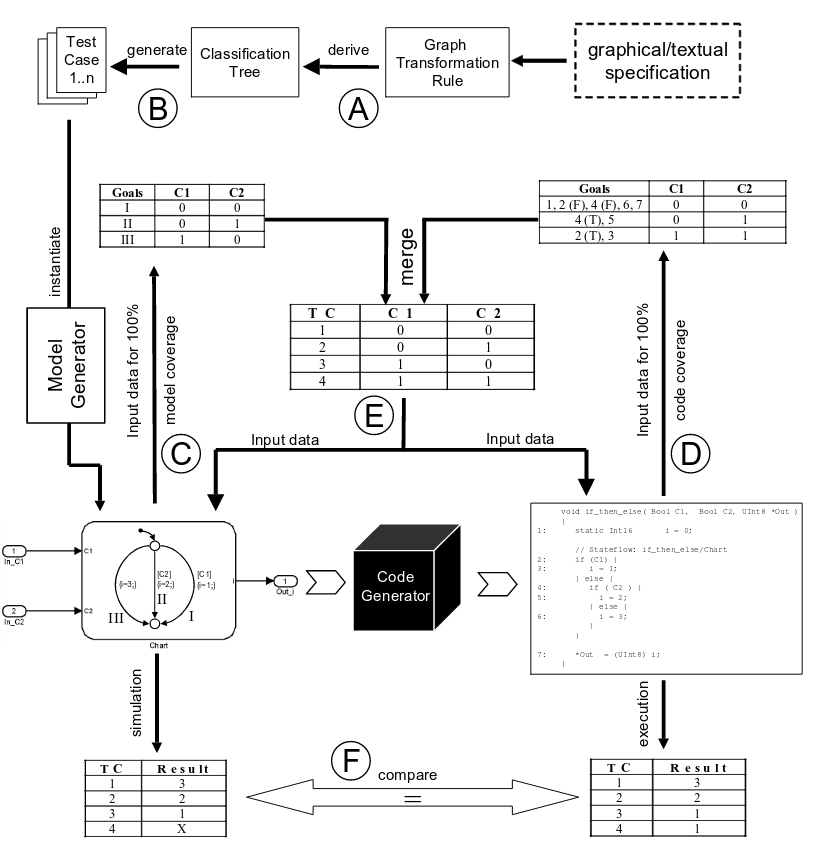
\includegraphics[width=0.7\linewidth]{images/codegen.png}
	\caption{Schéma de l'approche de Sturmer}
	\label{codegen}
\end{figure}

%Principaux points (json)

Cette solution possède le défaut d'être extrêmement dépendante du générateur à tester. Pour chaque générateur, il nous faut un oracle complexe
qui saura déterminer la sortie attendue en fonction du modèle. Nous avons voulu réaliser un logiciel de test qui soit facilement adaptable à des
projets différents ayant peu de choses en commun.

C'est pour cela que nous avons choisis de nous focaliser sur les dernières étapes, c'est à dire que
nous avons développer un logiciel qui prend en entrée un fichier contenant les instructions de générations et d’exécution du code ainsi que le résultat
attendu en fin d’exécution. Le but alors est de vérifier que le code généré produit bien le résultat attendu lors de l’exécution. La partie de génération
des cas de tests est laissé à l'utilisateur de notre logiciel. Cette approche est certes moins stricte qu'une analyse statique du programme générée par
le compilateur, comme le fait le compilateur XTend, mais permet d'obtenir des résultats tout aussi intéressants.

Nous fournissons deux modes pour tester un logiciel. Le premier mode est le plus simple, il suffit de fournir un fichier json bien formaté
ainsi que les fichiers nécessaires à la génération pour que le programme lance les tests et donne le résultat dans la console (cf Figure \ref{mode1}).

La seconde solution est plus contraignante, mais des développeurs courageux qui rechercheraient plus de précision ou de flexibilité dans les tests,
peuvent utiliser et étendre les interfaces de compilation et les parsers disponibles. Les résultats seront les mêmes néanmoins

\begin{figure}[!ht]
\begin{lstlisting}
francois@epona ~/insa/magienoire % java -jar Bubbles.jar sample.json
[1/4] : OK
[2/4] : OK
[3/4] : OK
[4/4] : FAIL
        expected : "Intended fail" but got : "\nHello world !!"
\end{lstlisting}
\caption{Utilisation du jar}
\label{mode1}
\end{figure}

%Software engineering

En ce qui concerne la gestion de projet, nous avons utilisé un dépôt Git pour la gestion de code étant donné que le CRI de l'INSA fournit une
instance de GitLab gratuitement aux étudiants avec un nombre illimité de dépôts privés. En ce qui concerne la documentation, puisque le code
est en \jv, nous avons utilisé la Javadoc, qui est générable par quiconque ayant un accès au code. Pour les itérations de développement,
nous avons développé les fonctionnalités de notre logiciel par couche et testé notre logiciel avec lui-même. Les tests ont évolués en même temps que le logiciel.
